\chapter{Metoder}
Dette kapitel indeholder beskrivelser af hvordan projektet er udført, og med hvilke metoder der er brugt. Yderligere indeholder kapitlet projektstyring, samt hvilke modeller der er fulgt igennem projektforløbet. 

\section{Samarbejdsaftale}
For at Gruppens medlemmer var enige fra starten af projektet, om blandt andet arbejdsindsats, samt timer der skulle bruges på projektet blev der lavet en samarbejdsaftale. Se samarbejdsaftalen i bilag XX

\section{Samarbejdspartnere}
Gruppens kunde er Søren Gregersen, overlæge på Medicinsk Endokrinologisk Afdeling, Aarhus Universitetshospital. Det er i samarbejde med Søren at projektet er blevet specificeret, samt hvilke krav der er til den endelige prototype.
Samuel Alberg Thrysøe er gruppens projektvejleder. Der er afholdt ugentlige vejledermøder, hvor gruppen har givet status på projektet og hvor der er diskuteret forskellige problemstillinger. 
Simon Vammen Grønbæk og Karl Johan Schmidt har fungeret som projektets review gruppe. Der er holdt møde hver tredje uge omhandlende aftalt dagsorden. Formålet med review gruppen er at få konstruktiv feedback på evt. rettelser, opbygning af rapport og generel forståelse. \fxnote{hvordan skal vi skrive mere til dette?}: gylle gylle: Til hvert vejledermøde har der været dagsorden med punkter, som formål og begrundelse for punktet på dagsorden. Dagsorden er sendt til vejleder senest en dag før vejledermødet, dette er gjort for at give vejleder en chance for at forberedelse sig på den givne dagsorden. Til hver vejledermøde er der udført et referat som kan ses i bilag XX. 

Reviewsmøderne har foregået på en lignede møde med vejledermøderne. Der er lagt en dagsorden for hver gruppe hvad der skulle reviews, hvor efter dokumenter er udvekslet mellem de to grupper. Grupperne har skrevet kommentar til dokumentet, hvorefter kommentarene og rettelserne er diskuteret på mødet. 

\newpage
\section{Versionsstyring}
I projektet er der gjort brug af versionsstyrings softwaren \textit{GitHub}. Til store ændringer har dokumenterne fået et nyt versions nummer og versionshistoriks tabellen er opdateret i hvert dokument se figur \ref{fig:versionsh}. 

\begin{figure}[H]
	\centering
	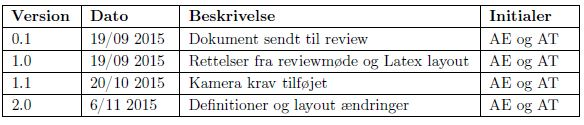
\includegraphics[width=1\textwidth]{billeder/Hovedrapport/versionshis.JPG}
	\caption{Versionshistorik tabel}
	\label{fig:versionsh}
\end{figure}

\subsection{GitHub}
Til versionsstyring af projektdokumentationen og source kode anvendes GitHub, som bygger på open source versions styrings systemet Git. Her opdateres der løbende ændringer, så det nyeste dokumentation og source kode altid er tilgængeligt. 
Som user interface til GitHub anvendes GitHub Desktop (figur: \ref{fig:git}). I GitHub Desktop vises en tidslinje, for hvornår der er lavet ændringer. Under de enkelte filer kan man se hvad der er ændret i for den gældende version. Programmet giver yderligere indblik i hvilke filer der lokalt er lavet ændringer i, som ikke er tilføjet repositoriet endnu.
\begin{figure}[H]
	\centering
	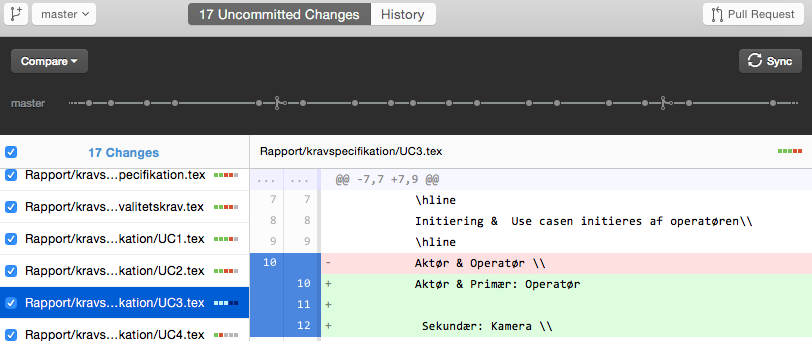
\includegraphics[width=1\textwidth]{billeder/github.png}
	\caption{GitHub Desktop}
	\label{fig:git}
\end{figure}
\newpage

\section{Projektstyring/planlægning} 
Til projektstyring af dette projekt er der brugt en stage gate model. En stage gage model(figur \ref{fig:stage-gate}) er bestående af nogle udviklingsfaser(stages), hvor ved der er en deadline for de konkrete faser. For at komme til næste fase/stage, skal der være opfyldt nogle kriterier. Kriterierne sættes op i en tjekliste(se figur \ref{fig:stage-gate-tjekliste}), hvor de kan krydses af. Alle punkter skal være opfyldt for at komme i gennem gaten. En stage gate model er god til at få et produkt på markedet, men det har sine svagheder ved en agil udviklingsprocess. \fxnote{skriv noget omkring at i dette projekt er gatene ikke lukkede efter de er gennem gået og derved kan der gåes tilbage og rettes i projektet}
\begin{landscape}
\begin{figure}[H]
	\centering
	\includegraphics[width=1.6\textwidth]{billeder/Hovedrapport/Stage-gateP.PDF}
	\caption{Stage gate model}
	\label{fig:stage-gate}
\end{figure}
\end{landscape}
\fxnote{stage gate modellayout}

\begin{figure}[H]
	\centering
	\includegraphics[width=0.7\textwidth]{billeder/Hovedrapport/Stagegatetjekliste.PDF}
	\caption{Stage gate model}
	\label{fig:stage-gate-tjekliste}
\end{figure}

%\begin{sidewaysfigure}
%\begin{figure}[H]
%	\centering
%	\includegraphics[width=0.6\textwidth]{billeder/Hovedrapport/Stage-gateP.PDF}
%	\caption{Stage gate model}
%	\label{fig:moscow}
%\end{figure}
%\end{sidewaysfigure}



%\begin{figure}
%  \begin{sideways}
%    \begin{minipage}{27.5cm}
%      \includegraphics[width=0.6\textwidth]{billeder/Hovedrapport/Stage-gateP.PDF}
%    \end{minipage}
%  \end{sideways}
%  \centering
%  \caption[Caption]{Caption.}
%  \label{pic:picture}
%\end{figure}

\subsection{Agil udviklingsprocess}
I projektet er der brugt en agil arbejdsprocess hvor der konstant fokus på at målrette og prioritere arbejdet mod det, der har givet mest værdi for projektet og kunden. Det vil sige at der løbende er prioriteret mellem opgaverne, hvorefter det er vigtigt at der hele tiden planlægges og revurdere delopgaverne. Det gør at projektets produkt og resultater evalueres og testes løbende, hvilket har dannet grundlag for prioritering af opgaverne der skulle løses i den næste periode. Til at sikre at arbejdsressourcerne der har været tilrådighed er blevet brugt på den mest effektive måde i projektet, er der brugt elementer fra SCRUM. SCRUM er en iterativ arbejdsmetode, hvor  der er iterationer(sprints), som i dette projekt har haft en periode på en uge. Til at holde styr på arbejdsressourcerne til opgaverne, har gruppen brugt \textit{Pivotaltracker}. 

I Pivotaltracker defineres projektets arbejdsopgaver, hvorefter de tildeles point alt efter hvor stor arbejdsbyrden er. De enkelte opgaver prioriteres herefter i projektets backlog, hvor Pivotaltracker automatisk tilføjer opgaver til den igangværende sprint udfra den nuværende “velocity”. En ny sprint påbegyndes automatisk når en ny uge starter.

Det betyder, at der er fuldstændig styr på om projektet går for langsomt, eller om udviklingen af projektet er godt med. Dette kan holdes op i mod den tidligere nævnte stage gate model.

Herudover giver Pivotaltracker mulighed for en komplet log over projektets udførte opgaver og afsluttede sprints. Her kan man se hvilke opgaver der er udført i hvilken uge. I projektet anvendes dette som logbog over udførte arbejdsopgaver.

En opgave kan have forskellige states, som definerer dens status. Når en opgave er afsluttet kan den afleveres til review, hvor den herefter enten kan godkendes eller afvises. Dette er særligt anvendeligt i projektets udviklingsfase, hvor en feature kan testes og godkendes af et andet projektmedlem. Figur \ref{fig:pt_sprints}  viser et overblik over tidligere sprints, hvor figur \ref{fig:pt_currentsprint} viser en igangværende sprint med opgaver der er godkendt, afsluttet og ikke færdiggjorte endnu.

\begin{figure}[htbp] \centering
\begin{minipage}[b]{0.48\textwidth} \centering
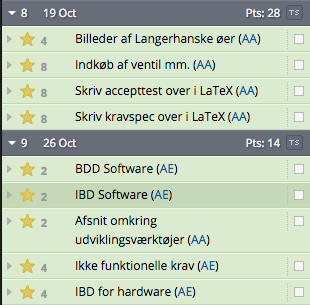
\includegraphics[width=1.00\textwidth]{billeder/pt_previous_sprints} % Left picture
\end{minipage} \hfill
\begin{minipage}[b]{0.48\textwidth} \centering
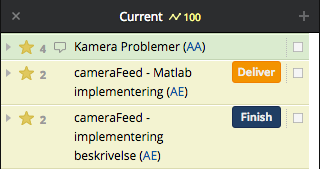
\includegraphics[width=1.00\textwidth]{billeder/pt_current_sprint} % Right picture
\end{minipage} \\ % Captions og labels
\begin{minipage}[t]{0.48\textwidth}
\caption{Færdiggjorte sprints} % Left caption and label
\label{fig:pt_sprints}
\end{minipage} \hfill
\begin{minipage}[t]{0.48\textwidth}
\caption{Igangværende sprint} % Right caption and label
\label{fig:pt_currentsprint}
\end{minipage}
\end{figure}
\fxnote{overvej om vi skal have andre billeder med en højere vilocity}

\section{De fire udviklingsfaser}
Under udviklingen af projektet, er der gennem gået fire faser. Den første fase i projektet har været koncept analyse. Koncept analysen bestod af litteratursøgning omkring langerhanske øer, dette blev gjort for at opnå tilstrækkelig viden omkring størrelserne, deres egenskaber mm. Der blev også søgt allerede eksisterende sorteringsmetoder, som blev anvendt på det daværende tidspunkt. Dette var primært for at opnå erfaring inden for området på kort tid. Efter litteratursøgningen blev et overordnet koncept etableret i samarbejde med kunden(\textit{Søren Gregersen}). Samtidigt med koncept analysen, blev det parallelt med tænkt på produktionen af produktet. Grunden til dette er, at det vil være uanvendeligt at opnå løsninger, som er for besværlige at producere. 

Den anden fase består af kravspecifikationen, hvilket er udarbejdet i tæt samarbejde med kunden. En kravspecifikation sikre at kunde og projekt udviklere er enige om projektets udformning. I kravspecifikationen er der brugt usecasediagram, samt fully dressed beskrivelser til hver usecase. Der laves fully dressed, for at klaregøre normal forløbet for hver usecase, samt undtagelser og udvidelser til dem. Derudover det også i kravspecifikationen at der er specificeret ikke funktionelle krav og kvalitetskrav. Samtidigt med kravspecifikationen er der udarbejdet en accepttest. Denne test er med til at verificere at alle krav, der er bestemt i samarbejde med kunde er opfyldte. I accepttesten er det beskrevet hvordan hver enkelt krav skal testes. Accepttesten udføres før produktet afleveres til kunden. Se afsnit \ref{subsec:krav} for eksempler.

Den tredje fase i projektet har været designfasen, hvor der udfra kravspecifikationen er lavet overordnede diagrammer. Diagrammerne bruges til at beskrive systemet overordnet, men også i små delsystemer. Det er diagrammerne der bruges til at videre udvikling af systemet. Desuden er de enkelte komponenters specifikationer beskrevet i designdokumentet. Derfor er det i denne fase der er bestilt komponenter til projektet. Se afsnit \ref{subsec:design} for eksempler. Efter denne fase blev det klart for gruppen, at der skulle bruges mere tid for at opnå målet defineret fra starten. Derfor blev der iværksat en handlingsplan for projektet, som kan ses i BILAG XX. De Primære dele af handlingsplanen består i øge arbejdsressourcerne til 50 timer i ugen. hvilket også kan ses i \textit{pivotaltracker}, hvor målet \textit{Velocity} har været 100point. 

I den fjerde fase er der blevet produceret en prototype. Derfor er der i denne fase kodet, monteret og testet. Denne fase er sket efter en iterativ proces, så der først kodes, monteres og derefter testes det. Dette er gjort ved så små delelementer som muligt, for at være sikker på at hver delelement virker inden det sættes sammen. Se afsnit \ref{subsec:Implement} for eksempler af denne fase. 

De fire udviklings faser brugt i projektet kan illustreres som på figur \ref{fig:v-model}. Modellen har sine fordele og ulemper. Fordelene er at der sikres dokumentation af projektet fra starten, samt at der hele tiden tænkes på slutresultatet og slutbrugeren. Ulemperne er at der er meget dokumentation, der bliver ændret fra hvad det var i starten af projektet. På den måde kan man godt tro at det er spild af tid, men det sikre samtidigt at projektet bliver vel dokumenteret og gennemtænkt fra starten.

\begin{figure}[H]
	\centering
	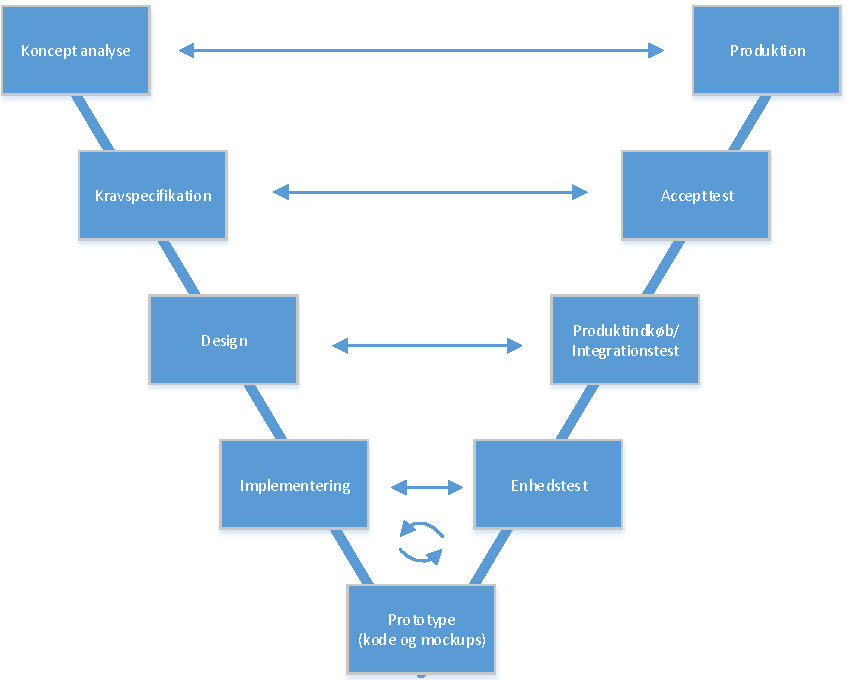
\includegraphics[width=0.7\textwidth]{billeder/Hovedrapport/V-model.PDF}
	\caption{Stage gate model}
	\label{fig:v-model}
\end{figure}

I modsætning til v-modellen findes der også vandfaldsmodellen, hvor hver enkelt fase bliver lavet færdig før næste fase påbegyndes. Dette medfører ofte nedprioritering af test og andre sene deadlines i projektet, grundet at tidligere tidsplaner er overskredet.



-samarbejdsaftaler

handlingsplan kontra tidsplan fra forprojektet

lavet efter design dokumentet er færdig bla bla bla. konrekte opgaver er lavet

- indsæt eksempel med loadcelle
